\section{Problem statement}

The Kapitza pendulum is a pendulum in which the pivot point oscillates up and down. Experimental observations show that, unlike a regular pendulum, this system can exhibit a stable fixed point in the inverted position (where the mass is directly above the pivot) in addition to the stable fixed point of the regular pendulum.

In particular, the pivot point oscillates with a frequency much greater than the characteristic frequency of oscillation of the pendulum. Let the 
$y$-coordinate of the pivot point be described as:
\begin{equation*}
    y_P = b \cos{\omega t}
\end{equation*}
and its acceleration as:
\begin{equation*}
    a_P = \dv[2]{y_P}{t} = -b \omega^2 \cos{\omega t}
\end{equation*}

This results in the following equation of motion for the system:
\begin{equation}
    \ddot{\theta} - \frac{1}{l} \left( g + b \omega^2 \cos{\omega t} \right) \sin{\theta} + c \dot{\theta} = 0
\end{equation}
where $\theta$ denotes the angle between the pendulum's arm and the vertical direction when the system is in the upper fixed point position, as shown in Figure \ref{fig:pendulum}. Here, $\omega \gg \sqrt{\flatfrac{g}{l}}$.

\begin{figure}[h]
    \centering
    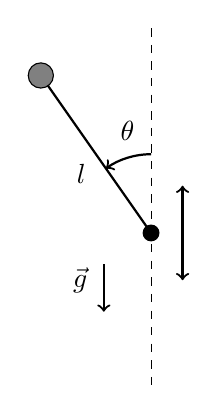
\begin{tikzpicture}[scale=2]
    
    % Define coordinates
    \coordinate (Pivot) at (0, 0.5); % Pivot point
    \coordinate (Mass) at (-0.7, 1.5); % Mass hanging at an angle
    
    % Draw the vertical pivot oscillating arrow
    \draw[<->, thick] (0.2, 0.8) -- ++(0, -0.6);
    
    % Draw the pendulum
    \draw[thick] (Pivot) -- (Mass) node[pos=0.5, below left] {$l$}; % Pendulum rod
    \filldraw[fill=gray] (Mass) circle (0.08cm) node[below] {}; % Mass as a gray circle
    
    % Draw angle
    \draw[thick, ->] (0, 1) arc[start angle=90, end angle=125, radius=0.5cm];
    \node at (-0.15, 1.15) {$\theta$};

    % Pivot point (oscillating point)
    \filldraw (Pivot) circle (0.05cm) node[above right] {};
    
    % Fixed vertical dashed line to indicate vertical position
    \draw[dashed] (0, 1.8) -- (0, -0.5);
    
    % Label for angle measurement
    \draw[->, thick] (-0.3, 0.3) -- ++(0, -0.3);
    \node at (-0.45, 0.2) {$\vec{g}$};
    
    \end{tikzpicture}
    \caption{Kapitza's pendulum.}
    \label{fig:pendulum}
\end{figure}


The equation can be rewritten highlighting the potential:
\begin{equation} \label{eq:kapitza_potential}
    \ddot{\theta} = -c \dot{\theta} - \pdv{V}{\theta}, \quad V(\theta, t) = \frac{1}{l} \left( g + b \omega^2 \cos{\omega t} \right) \cos{\theta}
\end{equation}

The dynamics of the system feature two distinct behaviours: the fast oscillations of the pivot point and the slow oscillations of the pendulum. Given this dual nature, the multiscale method is particularly well-suited to determine the system's trajectory.

To identify the actual free parameters of the system, it is useful to eliminate the physical units from the equation. The dimensionless form is given by:
\begin{equation}
    \ddot{\theta} - ( \sigma + a \cos{t'}) \sin \theta + \mu \dot{\theta} = 0
\end{equation}
where the parameters are defined as $\mu = \flatfrac{c}{\omega}$, $a = \flatfrac{b}{\omega}$, and $\sigma = \flatfrac{g}{l \omega^2}$. To apply the multiscale method, it is assumed that the parameters scale as $\mu \sim \epsilon$, $a \sim \epsilon$ and $\sigma \sim \epsilon^2$, where $\epsilon$ is a small parameter.

By applying the multiscale method, a solvability condition similar to the original equation (Eq \eqref{eq:kapitza_potential}) is obtained:
\begin{equation*}
    \ddot{\theta}_0 = - \mu \dot{\theta}_0 - \pdv{V_\text{eff}}{\theta}, \quad V_\text{eff}(\theta) = \sigma \cos \theta - \frac{a^2}{8} \cos 2 \theta
\end{equation*}
In this expression, the non-autonomous potential $V(\theta, t)$ is replaced by an effective autonomous potential $V_\text{eff}(\theta)$, which represents a time-averaged version of the original potential.
Stability of the fixed point $\theta = 0$ is determined by analysing the curvature of the effective potential at $\theta = 0$:
\begin{equation}
    \eval{\pdv[2]{V_\text{eff}}{\theta}}_0 = -\sigma + \frac{a^2}{2}
\end{equation}
The fixed point is stable if the curvature is positive, leading to the condition:
\begin{equation}
    \sigma < \frac{a^2}{2}
\end{equation}

The primary objective of this project is to investigate the numerical stability of the upper fixed point in the $(a, \sigma)$--plane and compare the results with the predictions obtained using the multiscale method.